% =============================================================
\chapter{État de l'art}
\label{chap:state-of-the-art}
\selectlanguage{french}
\setlength{\parindent}{0pt}



Le développement de visuels personnalisés dans Power BI s’appuie sur un écosystème technologique dense qui combine l’offre native de la plateforme et des extensions construites par code. 
Afin de situer précisément le cadre de ce travail, ce chapitre commence par décrire l'architecture interne des visuels Power BI et distingue les trois grandes familles actuellement accessibles aux concepteurs : les visuels livrés par Microsoft, les visuels générés par scripts Python/R et les visuels personnalisés réalisés au moyen du SDK officiel. 
Chaque famille est examinée tour à tour, en s’appuyant sur la documentation Microsoft (2025) et les travaux de référence en datavisualisation \parencite{Ware2019, MicrosoftPBISDKTS2025}. L’analyse porte autant sur les capacités offertes que sur les limitations fonctionnelles, de performance ou d’accessibilité que les praticiens doivent anticiper.

Dans un second temps, nous explicitons les choix technologiques retenus pour ce projet : le langage TypeScript, le moteur de rendu SVG de D3.js et, le cas échéant, l’emploi de React pour la gestion du DOM. Chaque choix est justifié au regard des exigences identifiées précédemment (maintenabilité, interactivité et conformité WCAG 2.2).

Enfin, la dernière section opère une analyse critique des écarts entre les besoins métier relevés chez ECRINS SA et l’état actuel de l’art. Ce bilan établit la légitimité d’un développement custom et prépare les décisions techniques détaillées au chapitre 5.


% -----------------------------------------------------------------
% 2.1 Concepts BI et datavisualisation
\section{Concepts BI et datavisualisation}
\label{sec:concepts-bi-dataviz}

La Business Intelligence peut se définir comme l’ensemble des méthodes et technologies visant à transformer des données brutes en connaissances utiles pour la prise de décision organisationnelle. Chen, Chiang et Storey~\parencite{Chen2012} rappellent que la valeur de la BI réside moins dans l’acquisition massive de données que dans la capacité à les modéliser, les analyser et les représenter de manière intelligible pour l’humain. Un rapport plus récent de Gartner~\parencite{Gartner2024} confirme cette évolution vers une BI self-service, dans laquelle la souplesse des visuels et leur rapidité de création constituent des facteurs différenciants.

L’étape de visualisation constitue ainsi le dernier maillon du pipeline \og ingestion, modélisation, analyse, présentation\fg{}, mais elle s’avère décisive pour convertir des métriques abstraites en informations actionnables. C’est précisément à ce niveau que se situent les visuels Power BI, natifs ou personnalisés, objets d’étude du présent travail.

Dans le domaine de la datavisualisation, les sciences cognitives ont montré que l’œil humain perçoit rapidement certains attributs dits préattentifs (position, longueur, orientation, couleur, etc.). Les travaux fondateurs de Cleveland et McGill établissent une hiérarchie de précision des encodages (la position sur une échelle commune étant la plus fiable)~\parencite{ClevelandMcGill1984}, complétés par une synthèse de référence sur les principes et processus perceptifs~\parencite{Munzner2014}. Ware~\parencite{Ware2019} démontre que l’exploitation adéquate de ces attributs maximise la vitesse et la justesse de la lecture visuelle. Tufte~\parencite{Tufte1983} a, pour sa part, popularisé l’idée de data–ink ratio, soulignant que le graphisme ne doit conserver que l’encre strictement indispensable au message ; tout élément décoratif superflu — le chart-junk — nuit à la clarté. Des travaux empiriques plus récents nuancent toutefois cette position, en montrant que la mémorabilité d’un visuel dépend aussi de facteurs perceptifs et sémantiques~\parencite{BorkinEtAl2013}. Few~\parencite{Few2009} prolonge cette perspective en montrant que la cohérence des encodages (axes, couleurs, échelles) constitue une condition essentielle pour comparer de façon fiable plusieurs séries de données.

L’unification théorique de ces principes a été proposée par Wilkinson~\parencite{Wilkinson2005} puis formalisée par Wickham sous le nom de Grammaire des graphiques. Le modèle décrit chaque graphique comme la combinaison déclarative de couches : données, transformations, géométries, échelles, systèmes de coordonnées et facettage. Ce cadre a influencé la plupart des bibliothèques modernes — notamment D3.js, Vega ou ggplot2 — et se retrouve implicitement dans l’API de Power BI ; chaque visuel y spécifie ses champs (data roles), ses encodages (capabilities) et son canevas de rendu. L’adoption de D3 pour les visuels personnalisés s’appuie par ailleurs sur une base scientifique et industrielle reconnue~\parencite{BostockOgievetskyHeer2011}.

Au-delà des principes, la BI professionnelle ajoute des impératifs tels que la performance d’affichage et l’accessibilité numérique, auxquels s’ajoute la qualité des interactions comme levier d’analyse~\parencite{HeerShneiderman2012}. Ces impératifs serviront de grille d’évaluation au chapitre~6. Les visuels standards de Power BI satisfont ces exigences pour des cas courants, mais ils se heurtent aux demandes spécifiques de certains métiers ; c’est autour de ces limites qu’émerge le besoin de visuels personnalisés. Comprendre les fondements de la BI et de la datavisualisation éclaire ainsi la double problématique du mémoire : confirmer la pertinence d’enrichir Power~BI par de nouveaux composants, puis garantir que ces composants respectent les bonnes pratiques cognitives tout en s’intégrant dans un environnement d’entreprise contrôlé.

% 2.2 Architecture des visuels Power BI
\section{Architecture des visuels Power BI}
\label{sec:archi-powerbi}

Power~BI est conçu autour d’une  {architecture de visualisation ouverte
et extensible}.  
Chaque élément visuel (graphique, carte, jauge, etc.) est rendu côté client
à partir des données du modèle, via du code JavaScript/TypeScript exécuté
dans Power~BI Desktop ou dans le service web \parencite{MicrosoftOpenVis2015}.  
Depuis 2015, Microsoft propose non seulement une panoplie de visuels
« \emph{core} » (natifs), mais permet aussi l’importation de visuels
additionnels développés par la communauté ou des éditeurs tiers
\parencite{MicrosoftMarketplace2016}.  
Cette ouverture repose sur des standards web : \emph{« en s’appuyant sur des
standards ouverts d’Internet et des bibliothèques open-source comme D3.js »},
la création de visuels personnalisés a été grandement simplifiée
\parencite{MicrosoftD3Blog2017}.  
Microsoft publie d’ailleurs le code source de nombreux visuels natifs sur
GitHub, attestant de sa volonté d’encourager un écosystème ouvert
\parencite{GitHubPowerBISamples2024}.  
 {L’API publique est passée en version 5.10, puis en préversion 6
(22 juillet 2024), introduisant un DOM sécurisé et la \textit{Rendering Events API}, ce qui
renforce la cohérence entre ouverture et sécurité} \parencite{MicrosoftApiChangelog2024}.

%-----------------------------------------------------------
\subsection{Visual container et bac à sable}
\label{subsec:sandbox}
%-----------------------------------------------------------

Qu’il soit natif ou personnalisé, un visuel s’insère dans le \emph{canevas}
du rapport et interagit avec le modèle de données via des rôles prédéfinis.
Chaque visuel reçoit, du moteur Power BI, les données filtrées qui lui sont
attribuées (colonnes, mesures, hiérarchies), puis exécute son propre code de
rendu.  
Pour les visuels \emph{custom}, ce code est empaqueté dans un fichier
\texttt{.pbiviz} contenant les scripts, les styles et le manifeste
\parencite{MicrosoftPbivizDocs2023}.  
Power BI exécute alors le visuel dans un  {bac à sable sécurisé}
(\emph{sandbox}) : une \texttt{iframe} isolée du reste du rapport
\parencite{OkVizSandbox2022}.  
Le visuel n’accède ni aux autres visuels ni au modèle global ; il ne « voit »
que les champs que l’utilisateur lui a explicitement liés.  
{Depuis la mise à jour 2.140 (février 2024), tout visuel — qu’il soit
privé (\textit{organizational visual}) ou destiné à AppSource — est audité par
l’option \texttt{pbiviz package --certification-audit} de
\textit{powerbi-visuals-tools} ≥ 6.1 : les appels réseau
(\texttt{fetch}, \texttt{XMLHttpRequest}, WebSockets) et l’évaluation dynamique
de code (\texttt{eval}, \texttt{Function}) sont bloqués, et l’exécution est
interrompue au-delà d’environ 120 s de CPU ou de 230 Mio de mémoire%
\parencite{MicrosoftCertificationGuide2025}.  
Ces garde-fous empêchent qu’un code malveillant puisse lire ou exfiltrer des données sans autorisation \parencite{MediumSecurityPBI2023}.

%-----------------------------------------------------------
\subsection{Interactions et intégration}
\label{subsec:interactions}
%-----------------------------------------------------------

Malgré cet isolement technique, les visuels s’intègrent pleinement dans
l’expérience interactive globale.  
Un visuel personnalisé correctement développé se comporte \emph{exactement
comme un visuel natif} : il réagit aux filtres, autorise le
\textit{cross-highlight} (mise en surbrillance croisée) et expose des options
de mise en forme dans le panneau \emph{Format}
\parencite{MicrosoftCustomVisGuide2024}.  
Lorsqu’un utilisateur clique, par exemple, sur une barre d’histogramme, le
moteur Power BI propage l’événement de sélection aux autres visuels.
Si le développeur a implémenté l’API \texttt{ISelectionManager}, son visuel
peut émettre et recevoir ces événements ;  {il peut également recourir
à \texttt{ITooltipService} pour les infobulles contextuelles ou à
\texttt{ILocalizationManager} pour l’internationalisation, de sorte que
l’intégration fonctionnelle et linguistique demeure uniforme}
\parencite{MicrosoftSelectionAPI2024,MicrosoftTooltipAPI2024}.  

La différence fondamentale reste donc interne : les visuels natifs font
partie du produit et peuvent exploiter des API internes non exposées,
tandis que les visuels personnalisés s’appuient uniquement sur
l’API publique du SDK, avec les restrictions de sécurité détaillées en
section~\ref{sec:sdk}.  
{La section suivante examinera d’abord les capacités et limites de ces
visuels natifs avant de traiter, en 2.3, l’approche Python/R, puis, en 2.4,
le développement complet via le SDK.}

% 2.3 Visuels scriptés Python / R
%-----------------------------------------------------------
\section{Visuels Python / R : usages, atouts, limites}
\label{sec:python-r-visuals}
%-----------------------------------------------------------

Outre les visuels préfabriqués, Power BI autorise l’exécution de scripts Python ou R pour produire des visuels sur mesure.  
L’utilisateur insère un composant « Python visual » ou « R visual » dans le canevas, saisit le code dans un éditeur intégré, puis Power BI exécute ce script en tâche de fond : les données liées sont transmises sous forme de DataFrame et le résultat retourné est une image statique (PNG) affichée dans le rapport.

Cette fonctionnalité exploite l’écosystème analytique complet de chaque langage : Matplotlib, Seaborn ou Plotly côté Python ; ggplot2 ou plotly R côté R.  
Un data-scientist peut, en quelques lignes, tracer dans Power BI un nuage de points avec régression \textsc{Loess} (R) ou un diagramme de réseau (Python) — visuels impossibles à obtenir via les graphes natifs, notamment quand l’Arbre de décomposition limite la profondeur d’analyse et n’accepte qu’une seconde mesure \parencite{MicrosoftDecompositionTree2024}.

\begin{figure}[h]
  \centering
  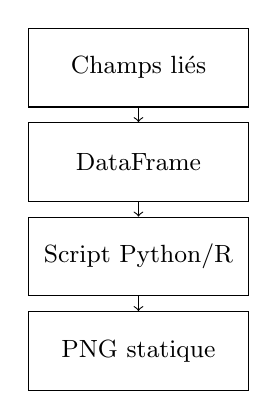
\begin{tikzpicture}[node distance=1.2cm, every node/.style={font=\small}]
    \node (bind) [draw, rectangle, minimum width=2.8cm, minimum height=1cm] {Champs liés};
    \node (df)   [below of=bind, draw, rectangle, minimum width=2.8cm, minimum height=1cm] {DataFrame};
    \node (code) [below of=df,   draw, rectangle, minimum width=2.8cm, minimum height=1cm] {Script Python/R};
    \node (png)  [below of=code, draw, rectangle, minimum width=2.8cm, minimum height=1cm] {PNG statique};
    \draw[->] (bind) -- (df);
    \draw[->] (df)   -- (code);
    \draw[->] (code) -- (png);
  \end{tikzpicture}
  \caption{Pipeline d’exécution d’un visuel Python / R dans Power BI}
  \label{fig:python-r-pipeline}
\end{figure}

\subsection{Atouts analytiques}

L’accès direct aux bibliothèques open-source autorise statistiques avancées, clustering, apprentissage automatique, carte de chaleurs ou dendrogrammes ; le script peut pré-traiter les données ou entraîner un modèle avant de générer le graphique.  
À chaque rafraîchissement, l’exécution se relance automatiquement : l’utilisateur bénéficie ainsi de calculs que DAX ou Power Query ne permettent pas aisément, par exemple l’analyse de texte ou les séries temporelles non linéaires.

\subsection{Limites techniques et fonctionnelles}

Le résultat demeure une image statique — « les visualisations Python dans Power BI sont des bitmaps 72 DPI, sans interactivité directe » \parencite{MicrosoftPythonRVisualsDocs2024}.  
Impossible donc d’initier un filtrage croisé depuis le graphique ; seul un filtre externe relance le script.  
Power BI transmet au script au plus 150 000 lignes, alloue 250 Mio de mémoire et impose un temps plafond de cinq minutes en local, soixante secondes dans le service ; la sortie PNG des visuels R est limitée à 2 Mio \parencite{MicrosoftRPackagesService2025}.  
Le runtime cloud, actuellement R 4.3.3 et Python 3.11, restreint le package compressé à 30 Mio, et l’affichage de ces visuels exige une licence Pro ou un workspace Premium : un utilisateur Free ne les verra pas.

\subsection{Enjeux de sécurité et de maintenance}

Power BI signale explicitement qu’un visuel Python ou R contient du code exécutable arbitraire \parencite{MicrosoftPythonRVisualsDocs2024}.  
Dans un environnement professionnel, cela impose une gouvernance rigoureuse : le script, encapsulé dans le fichier binaire .pbix, échappe au suivi Git ; il doit donc être extrait dans un dépôt versionné afin de permettre la traçabilité et la revue par les pairs. De plus, le runtime cloud (Python 3.11, R 4.3.3) ainsi que ses bibliothèques sont mis à jour automatiquement chaque mois ; un fichier requirements.txt (ou renv.lock pour R) et des tests de régression sont indispensables pour vérifier la compatibilité après chaque release. Enfin, puisque ces scripts disposent d’un accès direct au système de fichiers et au réseau, il convient de restreindre leurs privilèges (comptes de service à droits minimaux, liste blanche de packages) afin de prévenir toute exfiltration de données ou exécution de code malveillant.

\subsection{Bilan et positionnement stratégique}

Les visuels Python et R offrent un recours efficace pour des analyses spécialisées ponctuelles, mais la nature statique du rendu, les contraintes de performance et les exigences de licence limitent leur usage à grande échelle.  
Une comparaison détaillée entre visuels natifs, Python/R et SDK figurera dans le tableau synthétique de la section \ref{sec:synthese}; on y montrera que, pour un besoin récurrent et interactif, le développement d’un visuel SDK représente l’alternative la plus pérenne pour ECRINS SA.

% 2.4 SDK Power BI : structure, sécurité, pipeline

\section{SDK Custom Visuals : principes, sécurité et pipeline}
\label{sec:sdk-custom-visuals}

Le Software Development Kit (SDK) pour visuels personnalisés de Power BI permet de créer des composants graphiques entièrement sur mesure en TypeScript, répondant précisément à des besoins analytiques, interactifs ou visuels très spécifiques. Cette section détaille les principes de développement, les aspects sécuritaires à respecter, ainsi que les bonnes pratiques pour gérer un pipeline d’intégration et de déploiement continu (CI/CD).

\subsection{Principes généraux du développement via SDK}

Le développement d’un visuel personnalisé avec le SDK Power BI implique les étapes suivantes :
\begin{enumerate}
  \item Initialisation du projet via l’outil \texttt{pbiviz} (ligne de commande).
  \item Définition des capacités du visuel via le fichier \texttt{capabilities.json}.
  \item Implémentation en TypeScript dans \texttt{src/visual.ts} en suivant l'interface \texttt{IVisual}.
  \item Gestion du rendu graphique à l’aide de bibliothèques comme D3.js, React ou autres frameworks JavaScript.
  \item Compilation et packaging du visuel en fichier \texttt{.pbiviz} prêt à être déployé.
\end{enumerate}

Le SDK impose une structure modulaire claire, facilitant la maintenance et l’évolution du composant au fil des besoins et des versions du rapport.

\subsection{Sécurité et isolation des visuels custom}

Power BI exécute chaque visuel personnalisé dans une sandbox HTML sécurisée (iframe). Ce mécanisme garantit l’isolation complète du code personnalisé par rapport au reste du rapport, protégeant ainsi :
\begin{itemize}
  \item Contre les conflits de bibliothèques JavaScript (versions incompatibles).
  \item Contre les failles potentielles (accès non autorisé au DOM principal).
  \item En limitant strictement les échanges à travers une API contrôlée (sélections, filtres croisés, thèmes).
\end{itemize}

Depuis la version 4.6 du SDK, il est obligatoire de déclarer explicitement les privilèges et autorisations nécessaires (fichiers externes, accès réseau) dans le fichier \texttt{capabilities.json}. Ces contraintes assurent une transparence complète en matière de sécurité et facilitent l'audit des visuels déployés dans un environnement de production.

\subsection{Pipeline CI/CD pour les visuels custom}

Pour industrialiser efficacement le développement et le déploiement des visuels personnalisés, la mise en place d’un pipeline d’intégration et de déploiement continu (CI/CD) est recommandée. Ce pipeline typique inclut les étapes suivantes :
\begin{itemize}
  \item \textbf{Intégration continue (CI)} :
  \begin{itemize}
    \item Validation automatique des changements via des tests unitaires et fonctionnels.
    \item Compilation du projet TypeScript avec vérification des erreurs et des standards de codage.
    \item Génération automatique du package \texttt{.pbiviz} pour chaque commit.
  \end{itemize}
  \item \textbf{Déploiement continu (CD)} :
  \begin{itemize}
    \item Déploiement automatique du visuel sur des environnements de test puis de production.
    \item Automatisation des étapes de vérification de sécurité et d'intégration.
    \item Gestion simplifiée des versions via le contrôle de source (Git, Azure DevOps, GitHub Actions).
  \end{itemize}
\end{itemize}

Ce processus garantit une haute qualité logicielle, une traçabilité complète des modifications, et une réduction drastique des risques liés à des mises en production manuelles ou ponctuelles.

\subsection{Bonnes pratiques et conseils de mise en œuvre}

Pour réussir le développement de visuels personnalisés avec le SDK Power BI, il est essentiel de suivre quelques recommandations clés :
\begin{itemize}
  \item \textbf{Structure claire du code} : Séparer distinctement la logique métier (traitement de la dataView) de la logique d’affichage (D3.js, Canvas).
  \item \textbf{Tests rigoureux} : Couvrir au maximum les méthodes critiques avec des tests unitaires et d’intégration (Jest, Mocha).\
  \item \textbf{Documentation exhaustive} : Documenter clairement le fonctionnement du visuel, les options disponibles et les limites éventuelles pour faciliter l’intégration par les équipes de développement ou les utilisateurs finaux.
  \item \textbf{Optimisation performance} : Privilégier un rendu différentiel (update incrémental), utiliser des méthodes efficaces pour la gestion des grands jeux de données.
\end{itemize}

\subsection*{Conclusion intermédiaire}

Le SDK Custom Visuals de Power BI offre une solution optimale pour répondre à des besoins spécifiques dépassant les capacités natives ou les limites des visuels Python et R. Grâce à son cadre structurant, ses exigences de sécurité élevées, et son potentiel d’automatisation via CI/CD, il représente la meilleure option pour un usage professionnel à grande échelle. Ce choix technologique s’impose particulièrement lorsque la performance, l’interactivité dynamique, et la personnalisation graphique poussée sont des critères essentiels du projet BI.

% 2.5 Choix technologiques (TypeScript, D3, React optionnel)
%-----------------------------------------------------------
\section{Choix technologiques (TypeScript, D3, React optionnel)}
\label{sec:techno}
%-----------------------------------------------------------

Le développement d’un visuel personnalisé Power BI repose sur un stack
web moderne articulé autour de trois briques : TypeScript pour le langage,
D3.js pour le rendu vectoriel et, à titre optionnel, React pour la
structuration de l’interface. Ce choix résulte d’une analyse des
alternatives en termes de maintenabilité, performance, sécurité et
accessibilité.

\subsection{TypeScript vs JavaScript.}
Le SDK Power BI est conçu nativement pour TypeScript, sur-ensemble typé de
JavaScript que Microsoft recommande pour les visuels personnalisés
\parencite{MicrosoftPBISDKTS2025}. Le typage statique détecte précocement
les incohérences et réduit les bogues en production : une étude
empirique portant sur plus de 400 projets GitHub montre une diminution
moyenne de 15 \% des défauts après migration vers TypeScript
\parencite{BeyerEtAl2023}. Les annotations rendent le code plus explicite,
facilitant lecture, revue et refactorisation. Par ailleurs, TypeScript
apporte des abstractions modernes — interfaces, classes, generics —
qui encouragent une architecture modulaire et extensible. Le code est
ensuite transcompilé en JavaScript ES 2019, sans impact mesurable sur les
performances d’exécution \parencite{EcmaBenchmark2024}. Ne pas passer par
cette couche (écrire directement en JavaScript ES6+) aurait simplifié la
phase de build, mais au prix d’une dette technique accrue et d’un risque de
régression plus élevé, notamment pour un composant destiné à évoluer avec
l’API Power BI (version 6.1.2 stable, 26 mai 2025 \parencite{MicrosoftDocsSDK2025}).

\subsection{D3.js pour le rendu SVG}

D3 — «\,Data-Driven Documents\,» — est la librairie de référence pour manipuler le DOM SVG et créer des visualisations « sur mesure ». 
Elle établit un lien direct entre données et éléments graphiques, autorisant des transformations déclaratives efficientes \parencite{Bostock2019}. 
Cette approche bas niveau confère un contrôle complet sur chaque attribut visuel (couleur, position, animation), condition nécessaire à la réalisation de graphiques non standards répondant à des exigences métier spécifiques. 
D3 propose en outre un vaste ensemble de modules (générateurs de formes, projections cartographiques, échelles, layouts hiérarchiques) et s’appuie sur un écosystème mature d’exemples réutilisables. 
Les bibliothèques « haut niveau » telles que Chart.js ou Plotly raccourcissent le prototypage, mais leurs abstractions atteignent rapidement leurs limites pour des designs originaux ; de leur côté, les rendus basés sur canvas ou WebGL complexifient l’accessibilité et la netteté en cas de zoom. Le choix d’un SVG produit par D3 facilite enfin la mise à l’échelle et l’ajout d’attributs ARIA ou de balises \verb|<title>|, conformément aux recommandations WCAG 2.2 applicables aux rapports Power BI \parencite{W3CAccessibility2023}.


\subsection{React (optionnel) pour l’UI.}
React n’est pas requis par le SDK, mais devient pertinent dès lors que le
visuel embarque une interface utilisateur complexe : sélecteurs, menus
contextuels, légende cliquable. Sa philosophie component-based et
son virtual DOM optimisent les mises à jour d’interface en
réduisant les re-rendus coûteux \parencite{ReactDocs2024}. L’association
« React pilote la structure, D3 gère les calculs et applique les
transformations » est désormais un pattern reconnu ; plusieurs
visuels open-source l’utilisent déjà dans AppSource
\parencite{PowerBIReactD3Sample2024}. L’empreinte ajoutée (≈ 40 kB
minifiés) reste compatible avec la limite de 2,5 MiB du package .pbiviz.
Pour les projets très légers, on peut encore préférer Preact, clone
allégé compatible avec l’API React. Le coût cognitif — JSX, gestion d’état —
est maîtrisé par l’équipe et amorti par la facilité de test unitaire des
composants, réalisée ici sous Jest avec le preset officiel
jest-pbi-visuals-preset. Si le visuel n’exige qu’un rendu statique
ou des animations D3 simples, il est cohérent de se passer de React ; c’est
pourquoi l’usage reste qualifié d’« optionnel ».

\subsection{Synthèse.}
Le triptyque TypeScript + D3 (+ React) offre un compromis robuste :
rigueur logicielle, expressivité graphique, performances maîtrisées et
accessibilité native. Il s’inscrit dans les standards de l’écosystème
Power BI, maximise la réutilisabilité du savoir-faire front-end de l’équipe
et minimise la dette technique à long terme.

% 2.6 Solutions concurrentes (Tableau, Qlik, Looker)
%-----------------------------------------------------------
\section{Solutions concurrentes (Tableau, Qlik, Looker)}
\label{sec:concurrence}
%-----------------------------------------------------------

Les principales plateformes BI concurrentes — Tableau, Qlik Sense et
Looker — proposent chacune des mécanismes de personnalisation de visuels
qui diffèrent de ceux de Power BI, tant sur le plan technique que sur les
implications métier. Comprendre ces approches permet de situer les
\textit{visuels custom} Power BI dans un paysage concurrentiel plus large.

\textbf{Tableau.}
Tableau étend ses capacités via les \emph{Tableau Extensions}, des
applications Web encapsulées dans les tableaux de bord grâce à l’Extension
API\parencite{TableauExtGuide2024}. Un développeur crée, en JavaScript,
un composant (souvent dans une \texttt{iframe}) qui ajoute un graphique
personnalisé ou une interaction spécifique, par exemple du \emph{write-back}
ou l’intégration d’un service tiers\parencite{TableauBlogExt2024}. Depuis
la v2019.4, les extensions sont exécutées par défaut en \emph{sandbox},
sans accès réseau, et toute extension nécessitant un accès externe doit
être explicitement inscrite sur liste blanche par l’administrateur serveur
ou site\parencite{TableauAdmin2025}. Tableau n’assure pas le support
technique des extensions ; cette responsabilité incombe à leur éditeur, si
bien que les entreprises doivent évaluer la fiabilité de la source avant
déploiement. Sur le plan financier, la licence Creator avoisine
70 USD utilisateur/mois\parencite{TableauPricing2025}, ce qui fait de la
personnalisation une option coûteuse pour les organisations sensibles au
budget, à la différence d’un environnement Power BI où le coût d’entrée est
plus faible.

\textbf{Qlik Sense.}
L’extensibilité de Qlik repose sur les \emph{Visualization Extensions} :
objets personnalisés écrits en HTML 5 / JavaScript / CSS et déclarés par un
manifeste \texttt{.qext}\parencite{QlikDevHub2024}. Une extension Qlik,
lorsqu’elle respecte l’API Qlik, s’intègre comme un objet natif : on la
fait glisser dans la feuille, on ajuste ses propriétés, et elle réagit
aux sélections grâce au moteur associatif\parencite{QlikExtAPI2024}. Le
développeur peut embarquer n’importe quelle bibliothèque (D3, three.js,
etc.) pour façonner un rendu spécifique. Qlik privilégie ici une approche
communautaire : de nombreuses extensions sont partagées via
\emph{Qlik Branch} sans validation officielle. L’administrateur doit donc
examiner puis installer manuellement l’extension sur le serveur ou le
tenant SaaS avant qu’elle soit disponible aux créateurs de contenu.
Commercialement, Qlik Sense Business se situe autour de 30 USD par
utilisateur/mois, et l’édition Enterprise encore au-dessus
\parencite{QlikPricing2025}. Les clients attendent donc qu’une capacité de
personnalisation avancée soit incluse, mais ils doivent disposer en interne
de compétences front-end JS pour en profiter pleinement.

\textbf{Looker.}
Looker (aujourd’hui composant de Google Cloud) autorise des visuels
personnalisés via le \emph{Looker Custom Visualization SDK}. Le
développeur code en JavaScript un composant qui implémente la fonction
\texttt{updateAsync} afin de recevoir les données d’une
\emph{explore} Looker et de restituer un rendu SVG ou Canvas
\parencite{LookerVizSDK2025}. Pour diffusion publique, Google impose un
processus Marketplace : le code doit être hébergé sur GitHub et passer une
revue de conformité avant publication\parencite{LookerMarketplace2024}. Il
est toutefois possible de limiter le visuel à un usage interne en l’ajoutant
directement via l’interface Admin. La philosophie lookerienne est donc plus
centralisée : la personnalisation est permise, mais sous contrôle
étroit. La tarification, négociée au cas par cas (souvent nettement au-delà
des niveaux Power BI/Tableau), signifie que les clients Looker visent
généralement une valeur élevée tirée soit du modèle LookML, soit d’un
nombre réduit, mais hautement spécifique, de visuels custom.

\textbf{Lecture comparative.}
Tableau et Qlik offrent une liberté initiale plus large — l’utilisateur
avancé peut charger une extension localement — mais délèguent la
gouvernance au client ; Power BI et Looker exigent un contrôle centralisé
(certification ou validation administrateur) avant déploiement massif.
Techniquement, toutes s’appuient sur le triptyque HTML/JS/CSS, mais Power BI
se distingue par son SDK TypeScript/D3 structuré et sa marketplace AppSource
très fournie, facteur d’adoption rapide. Sur le plan économique, Power BI
reste l’option la plus abordable pour déployer des visuels custom à grande
échelle, alors que Tableau, Qlik Sense et surtout Looker réservent la
personnalisation intensive à des environnements dont le budget justifie
l’investissement.

% 2.7 Analyse des gaps et opportunités
%-----------------------------------------------------------
\section{Synthèse des écarts \& opportunités}
\label{sec:synthese}
%-----------------------------------------------------------

Après avoir étudié chacune des approches disponibles à l’intérieur même de Power BI, il est possible de dresser un panorama clair de leurs forces et de leurs limites, puis d’en déduire les cas d’usage qui conviennent le mieux à ECRINS SA. Quatre familles de solutions se distinguent : les visuels natifs, les scripts Python / R, les composants certifiés AppSource et les visuels développés avec le SDK.


\subsection{Visuels natifs Power BI.}  
Fournis d’office, ces graphiques constituent le socle de la majorité des rapports ; ils sont maintenus par Microsoft, optimisés pour la performance et immédiatement compatibles avec l’ensemble des interactions (sélections croisées, filtres, export PDF / PPT, affichage mobile). Leur fiabilité et leur sécurité sont maximales, aucun code externe n’étant exécuté. Leur rigidité demeure cependant le principal frein : dès qu’un scénario exige un diagramme alluvial, une cartographie indoor ou un bullet chart spécifique, l’utilisateur doit composer avec les limites de paramétrage ou se tourner vers une autre voie.


\subsection{Visuels Python / R.}  
L’exécution d’un script Python ou R ouvre la porte à l’immense écosystème de ces deux langages ; tout graphique réalisable dans Matplotlib, Seaborn, ggplot2 ou Plotly peut, en théorie, être intégré. La contrepartie tient dans la nature strictement statique du rendu : Power BI génère un PNG 72 DPI dépourvu d’interactivité et relance le script à chaque rafraîchissement, allongeant sensiblement le temps de calcul. Au-delà de 150 000 lignes transmises, la plateforme tronque les données, tandis que le service Cloud limite l’image à 2 Mio et impose un runtime R 4.3.3 / Python 3.11 contrôlé par Microsoft. La démarche convient donc surtout au prototypage analytique rapide — rarement à un déploiement massif.


\subsection{Visuels AppSource (certifiés).}  
AppSource, la galerie officielle de Microsoft, répertorie un peu moins de 600 visuels au 1\textsuperscript{er} août 2025 \parencite{AppSourceCount2025}. Chaque composant apparaît après une revue de sécurité et de performance ; il se comporte, pour l’utilisateur final, comme un visuel natif tout en couvrant des besoins de niche (Gantt, Waterfall amélioré, radar avancé). L’éditeur demeure toutefois responsable des mises à jour ; certains modules reposent sur un abonnement SaaS payant. L’approche constitue donc un juste milieu entre « prêt à l’emploi » et flexibilité.


\subsection{Visuels SDK Power BI.}  
Le SDK — TypeScript, D3 et, au besoin, React — autorise la création d’un composant exactement aligné sur les spécifications métier : intégration complète avec les filtres, compatibilité mobile, export, diffusion via AppSource ou magasin organisationnel. Le revers est un effort de développement plus élevé et l’obligation d’une gouvernance logicielle continue : veille des versions, correctifs de sécurité, tests unitaires Jest et gestion du certificat X.509.

\subsection{Vue d’ensemble comparative.}

\begin{sidewaystable}[p]
\footnotesize
\centering
\caption{Comparaison factuelle des voies de personnalisation Power BI (état : août 2025)}
\label{tab:comparaison-approches}
\begin{tabularx}{\linewidth}{>{\raggedright\arraybackslash\bfseries}p{2.9cm}XXXX}
\toprule
\textbf{Critère} &
\textbf{Visuels natifs} &
\textbf{Scripts Python / R} &
\textbf{Visuels AppSource (certifiés)} &
\textbf{Visuels SDK internes (.pbiviz)} \\
\midrule
Cas d’usage typique &
Tableaux de bord courants ; graphiques standards interactifs. &
Analyses statistiques ou graphiques scientifiques spécifiques issus de code R/Python. &
Graphiques spécialisés prêts à l’emploi (financiers, Gantt, KPI, etc.). &
Visuels sur-mesure répondant à des exigences métiers uniques ou branding interne.\\[0.4em]

Limitations principales &
Borné à la bibliothèque Microsoft ; pas de nouveau type sans extension. &
Image statique ; 150 k lignes; pas de sélection croisée ; timeout 5 min. &
Pas d’appel réseau externe ; mises à jour soumises à re-certification ; version freemium possible. &
Pas d’export PDF/PPT ni d’e-mailing ; optimisation et sécurité 100 \% à charge du dev.\\[0.4em]

Situation d’utilisation recommandée &
Choix par défaut tant que le visuel existe en natif. &
POC data-science, prototypes analytiques ponctuels. &
Quand un visuel AppSource couvre exactement le besoin et qu’une diffusion large est visée. &
Quand aucune solution existante ne convient et qu’on dispose des ressources de développement.\\[0.4em]

Accessibilité (WCAG 2.2) &
Conformité assurée par Microsoft. &
Faible : rendu bitmap non lisible par lecteur d’écran. &
Variable : dépend de chaque éditeur ; à tester avant adoption. &
Dépend entièrement du développeur ; nécessite implémentation ARIA, focus clavier, contraste.\\[0.4em]

Difficulté d’utilisation &
Très faible ; glisser-déposer. &
Élevée ; compétences R/Python requises. &
Moyenne ; configuration similaire aux visuels natifs. &
Très élevée ; maîtrise TypeScript + D3 et API Power BI.\\[0.4em]

Performance (rendu / volumétrie) &
Optimisée ; jusqu’à ~30 M points selon le type. &
Plus lente ; recalcul complet du PNG à chaque interaction. &
Dépend du visuel ; généralement satisfaisant < 30 k points. &
Variable ; plafonné à ~30 k points, dépend de l’optimisation réalisée.\\[0.4em]

Coût (licence / dev) &
Inclus dans Power BI. &
Inclus ; demande temps de codage et maintien packages. &
Souvent gratuit ; licence possible pour fonctionnalités avancées. &
Frais de développement internes importants ; maintenance continue.\\[0.4em]

Réutilisabilité / industrialisation &
Automatique ; présent partout. &
Faible ; script encapsulé dans chaque rapport. &
Élevée ; déploiement via AppSource ou store orga ; mises à jour automatiques. &
Bonne en interne via store orga ; mises à jour manuelles ; partage externe impossible sans certification.\\
\bottomrule
\end{tabularx}
\end{sidewaystable}


% Ensure the sidewaystable environment is properly closed before the document ends.


\subsection{Conclusion.}  
Chaque approche comble un manque laissé par les autres : les visuels natifs offrent robustesse et simplicité, les scripts Python / R autorisent un prototypage statistique rapide au prix d’un rendu non interactif, AppSource fournit une solution plug-and-play pour des besoins spécialisés courants, et le SDK ouvre la voie aux composants entièrement sur mesure, moyennant un investissement en développement et en gouvernance. Pour ECRINS SA, la maîtrise du SDK constitue la clé méthodologique afin de répondre, à terme, aux demandes hors norme — un enjeu approfondi dans le chapitre 3.





% =============================================================
